\documentclass[11pt]{beamer}
\usetheme{Warsaw}
\usepackage[utf8]{inputenc}
\usepackage[brazil]{babel}
\usepackage[T1]{fontenc}
\usepackage{amsmath}
\usepackage{amsfonts}
\usepackage{amssymb}
\usepackage{listings}

\lstdefinestyle{customc}{
  belowcaptionskip=1\baselineskip,
  breaklines=true,
  frame=L,
  xleftmargin=\parindent,
  language=C,
  showstringspaces=false,
  basicstyle=\tiny\ttfamily,
  keywordstyle=\bfseries\color{green!40!black},
  commentstyle=\itshape\color{purple!40!black},
  identifierstyle=\color{blue},
  stringstyle=\color{orange},
}

\lstset{escapechar=@,style=customc}



%Configuração do bloco de texto
\setbeamercolor{block title}{fg=white,bg=blue!75!black}

%inserir imagens
\usepackage{graphicx}

%inserir pdf
\usepackage{pdfpages}

\author{Augusto Ribas, Bruno Nazário, Doglas Sorgatto, Thiago Machado}
\title{Sistema de arquivos exFAT (Extended File Allocation Table)}

%\setbeamercovered{transparent}
%\setbeamertemplate{navigation symbols}{}
%\logo{}

\institute{Sistemas Operacionais}
\date{25/10/2014}

%\subject{}
\hyphenation{pro-du-to re-qui-si-tos pro-je-to or-ga-ni-za-cio-nal}

\begin{document}

\begin{frame}
\titlepage
\end{frame}

\begin{frame}{Visão Geral}
\scriptsize\tableofcontents
\end{frame}

\section{Introduçao}

\subsection{Introdução}
\begin{frame}{Introdução}
O exFAT (Extended File Allocation Table) é o sistema de arquivos da Microsoft optimizado para flash drives. É um sistema propretario e patentiado.\\
Esse sistema pode ser usado onde o NTFS não é uma solução viavel ou onde o limite do sistema padrãao FAT32 não é aceitavel.
\end{frame}

\subsection{Origem}
\begin{frame}{Origem}
exFAT começou como parte do Windows CE (Windows para sistemas mobile, de 1996, precursos do Windows Phone). Otimizando o uso de discos SSD.

\begin{center}
 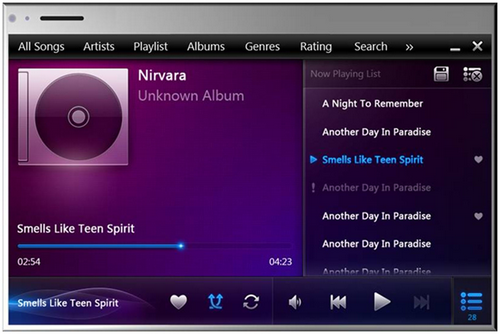
\includegraphics[width=0.5\textwidth]{WindowsCE7.png}
\end{center}
\end{frame}

\subsection{Para que outro sistema de arquivos?}
\begin{frame}{File systems optimized for flash memory, solid state media}
Discos de estados solidos (Solid state media), como memorias flash, são similares a discos quanto a suas interfaces, mas possuem problemas diferentes. No nivel mais baixo, eles requerem tratamento especial como diferentes algoritimos de tratamentos de erros. Tipicamente, um dispositivo como um solid-state disk lida com tais operações internamentes e assim um sistema de arquivo regular pode ser usado. Entretanto para certas instalações especializadas (como sistemas embarcados), um sistema de arquivos otimizado para o disco é necessario.

\begin{center}
 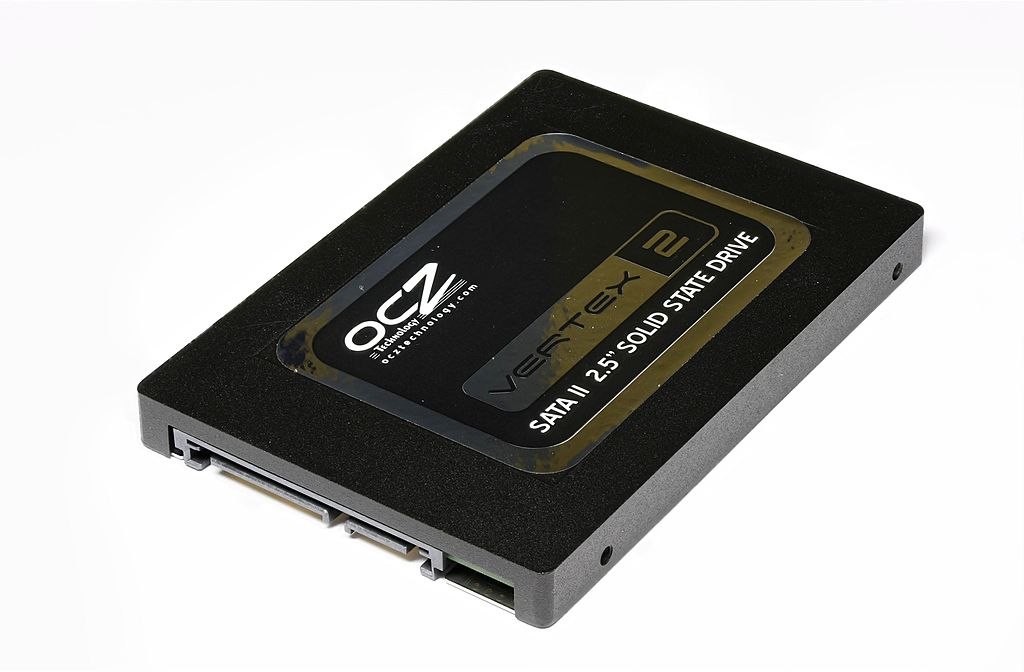
\includegraphics[width=0.3\textwidth]{sata1.jpg}
  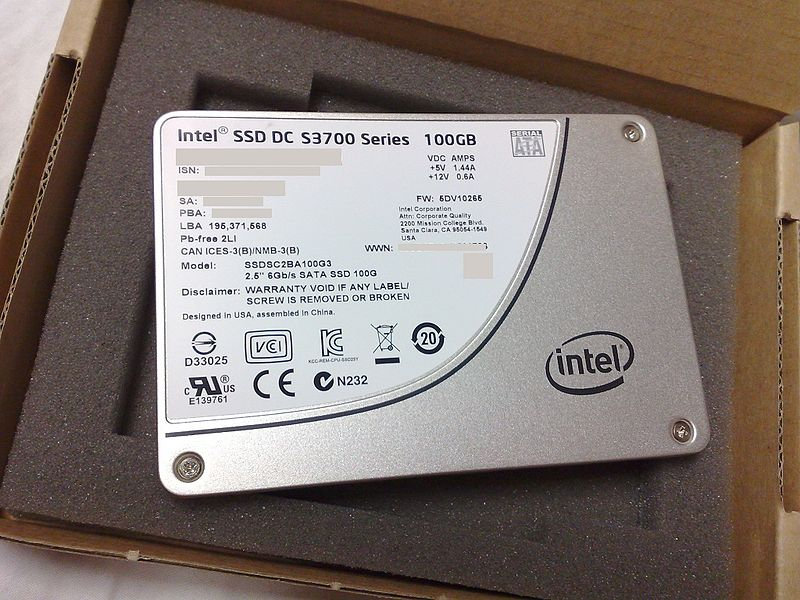
\includegraphics[width=0.3\textwidth]{sata2.jpg}
\end{center}

\end{frame}


\begin{frame}{Motivação}
O exFAT permite arquivos individuais maiores que 4 Gigabytes, facilitando a gravação de de videos longos em HD, que podem exceder 4Gb em menos de uma hora. Cameras usando Fat32 vão quebrar os arquivos de video em multiplos segmentos de 2 a 4 Gb. Com o aumento  de capacidade e dos dados sendo transferidos, a operação de escrita precisa ser feita de forma mais eficiente.
\end{frame}

\begin{frame}{Motivação}
SDXC(Secure Digital eXtended Capacity, especificação de armazenamento de dados para disco sd) cards, rodando UHS-1 tem uma velocidade minima garantida de 10MBps e o exFAT tem um papel importante em reduzir a sobrecarga na alocação de blocos (cluster). Isso é possivel  através da introdução do blocos(cluster) de bitmap e eliminação (ou redução) das escritas em tabela FAT. Um unico bit (flag) no registro de diretorio é usado para informar ao driver de disco exFAT quando um arquivo é continuo.
\begin{center}
 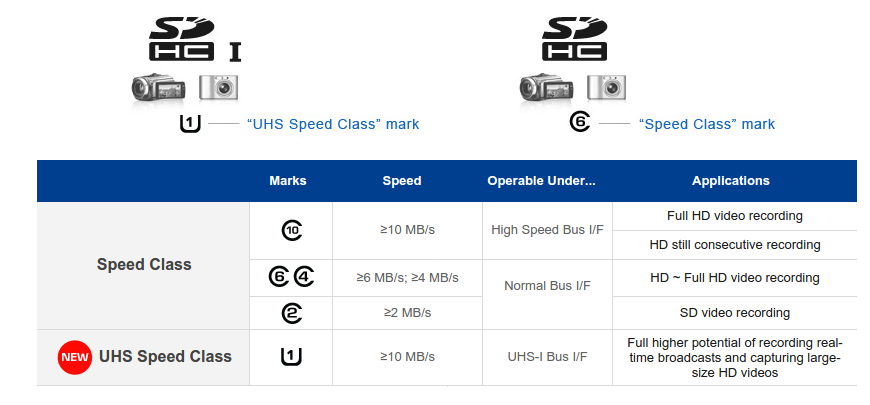
\includegraphics[width=0.5\textwidth]{uhs1.png} 
\end{center}
\end{frame}



\subsection{Mercado}
\begin{frame}{Comercialização}
Alguns vendedores de discos e memorias, incluindo os da pendrives USB, memoria flash e solid state drives (SSD) tem mandado de fabrica esses dispositivos pre-formatados com o sistema de arquivos exFAT.

\begin{center}
 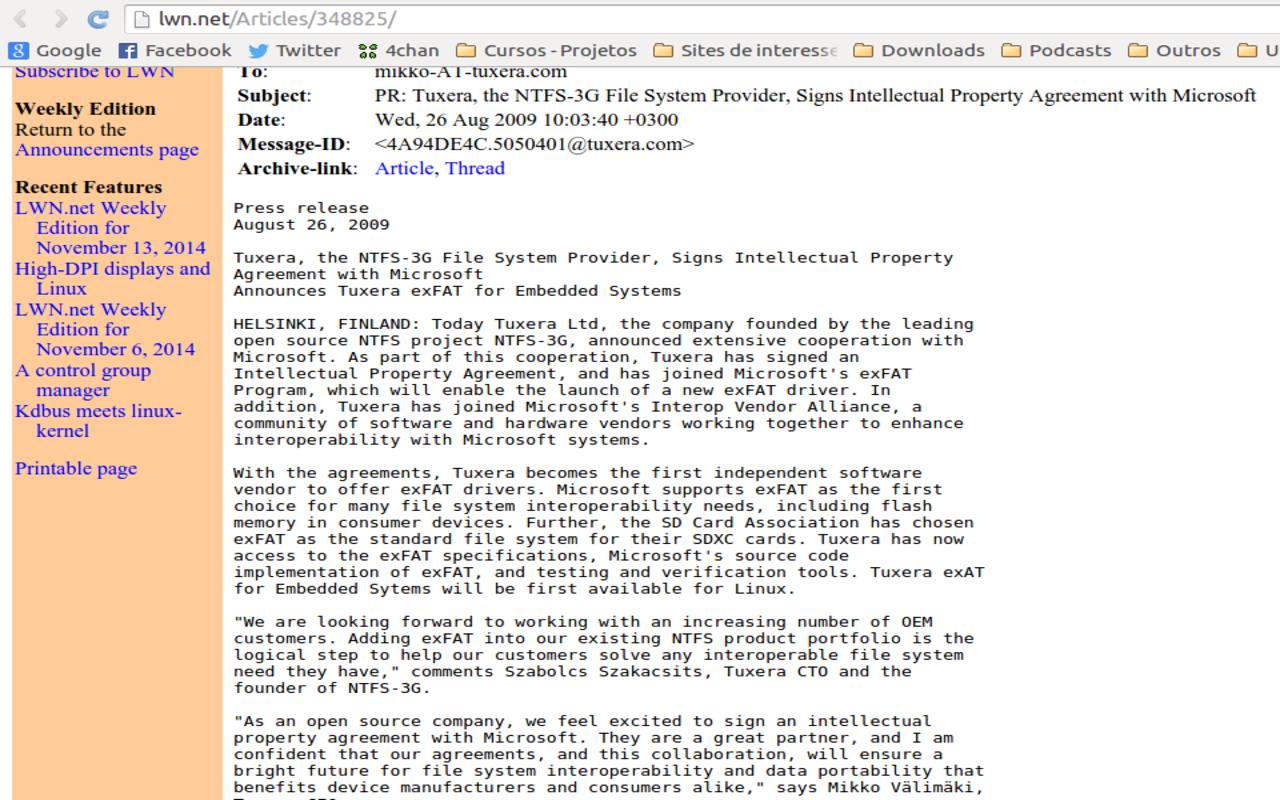
\includegraphics[width=0.5\textwidth]{tuxeraemail.png}
\end{center} 
\end{frame}

\begin{frame}{Adoção}
exFAT tem suporte no windows (XP, server 2003, CE 6.0, Vista, server 2008, 7, 8), Mac OS X Lion, OS X Mountain Lion, OS X Maverics e OS X Yosemite.

Companias podem integrar o exFAT em um grupo especifico de dispositivos para usuarios, incluindo cameras, filmadoras, porta retrados digitais, smartphones, pcs e redes por um preco variavel.

A microsoft entrou com acordos de licenciamento com a BlackBerry, Panasonic, Sanyo, Canon, Aspen Avionics e BMW.
\end{frame}

\begin{frame}{Adoção}
Uma implementação FUSE-based (Filesystem in Userspace) chamada de fuse-exfat ou exfat-fuse, com funções de leitura e escrita esta diponivel para FreeBSD e distribuições linux. Uma implementação para o kernel também foi feita pela Samsung. ela foi liberada no pelo github inicialmente, mas de forma nao intencional, sendo posteriormente liberada oficialmente pela Samsung com uma licenca GPL. No entando nenhuma das soluções  pode ser incorporada oficialmente ao kernel do linux devido as patentes da Microsoft com relação ao exFAT.
\end{frame}

\begin{frame}{Adoção}
Soluções proprietaria de escrita e leitura licenciadas e derivada da implementação da Microsoft são disponiveis para Android, Linux e outros sistemas operacionais pela Paragon Software Group e Tuxera.
\begin{center}
 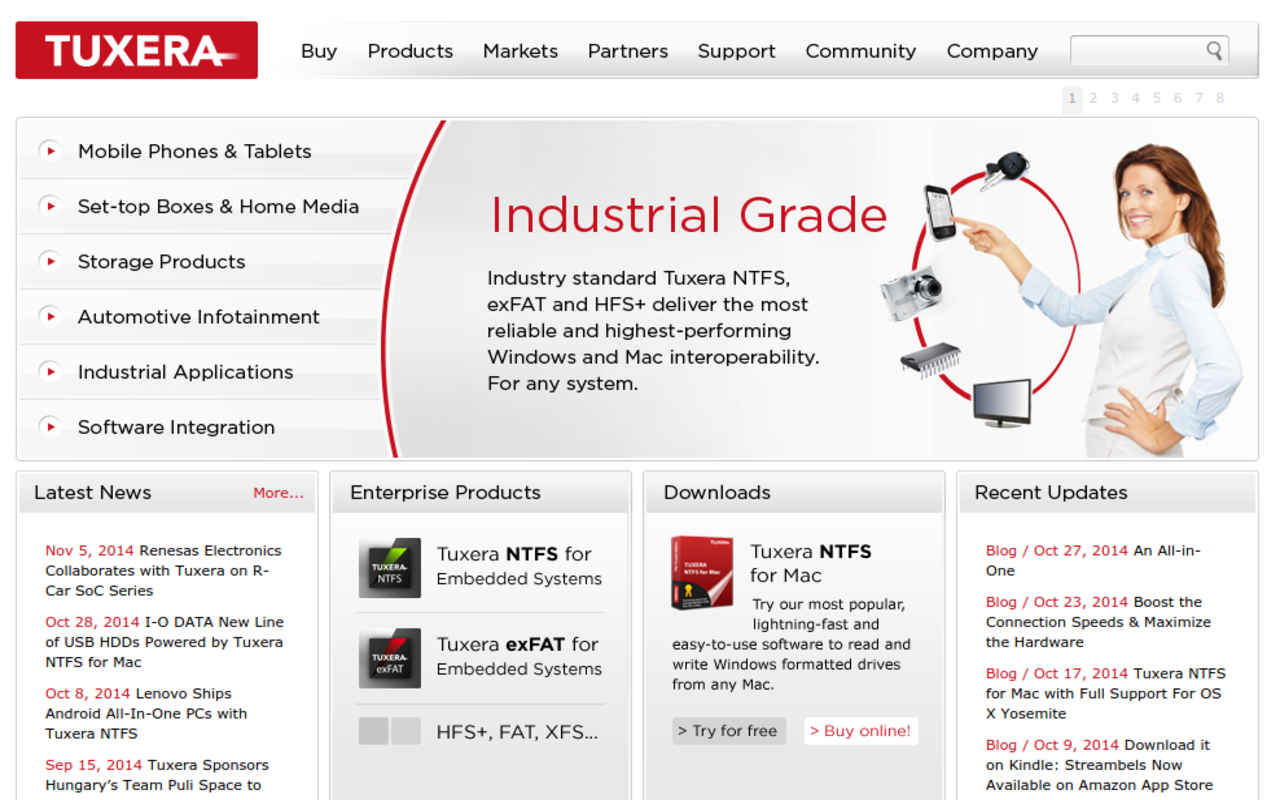
\includegraphics[width=0.5\textwidth]{tuxerasite.png} 
\end{center}
\end{frame}

\section{Especificações Tecnicas}

\begin{frame}{Localização de nome de arquivo}
Em 2012, a microsoft ganhou a patente US8321439, referente ao "Quick File Name Lookup Using Name Hash", que é o algoritimo usado no exFAT para acelerar a procura por nomes de arquivos.
\begin{center}
 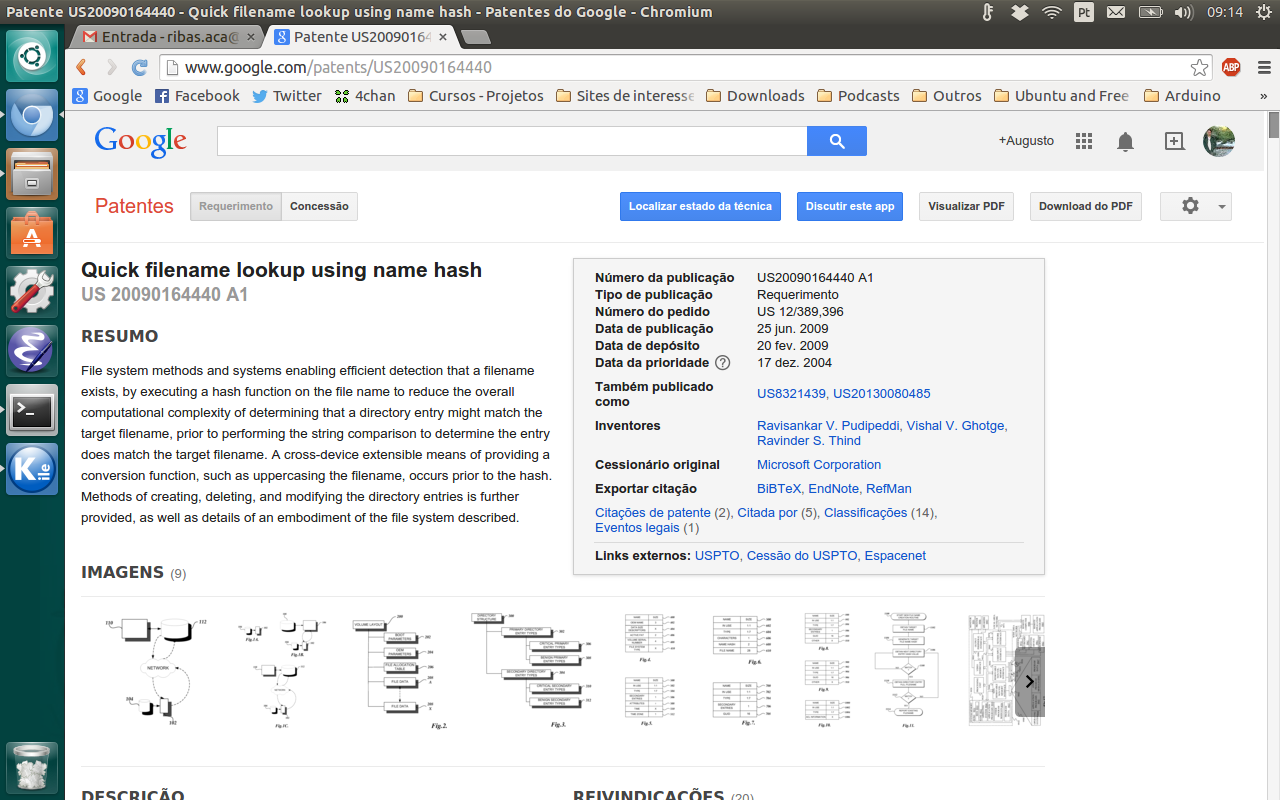
\includegraphics[width=0.5\textwidth]{quicksearch.png} 
\end{center}
\end{frame}

\begin{frame}{Pré-alocação de Arquivo e Cluster}
Como o NTFS, o exFAT pre-aloca espaço em disco para um arquivo apenas marcando um espaço arbritario no disco como "alocado". Para cada arquivo, o exFAT usa dois campo separados de 64 bits no diretorio, o VDL (Tamanho valido de dados, ou Valid Data Length), que indica o tamanho real do arquivo, e o tamanho fisico dos dados (physical data length).
Para melhorar a alocação de blocos (cluster) para o armazenamento de um novo arquivo, a Microsoft incorporou um método de pre-alocação-contigo para blocos (cluster) que ignora a tabela FAT.
\end{frame}

\begin{frame}{Pré-alocação de Arquivo e Cluster}
Uma caracteristica do exFAT (usada no exFAT para sistemas embarcados) prove transações atomicas para o update os metadados do sistema de arquivos em multiplos passos, essa caracteristica chamada de Transaction Safe FAT (TexFat).
\begin{center}
 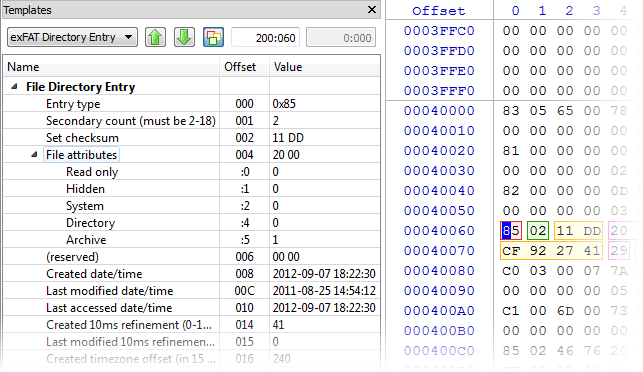
\includegraphics[width=0.35\textwidth]{entradaexfat.png} 
\end{center}
http://www.disk-editor.org/
\end{frame}

\begin{frame}{Directory file set}
exFAT e o resto da familia FAT para sistemas de arquivos não usa indices por nomes de arquivos, diferente do NTFS que usa arvores B para a procura de arquivos. Quando um arquivo é acessado, o diretorio preecisa ser buscado sequencialmente até que um a busca produza um resultado. Para nomes de arquivos menores que 16 caracteres, um registro de nome é requerido, mas o nome do arquivo é representando por tres registros de diretorios de 32 bytes. Isso é chamado de "directory file set", e um diretorio de 256 MiB pode ter até 2,796,202 nomes de arquivos. (Se arquivos tiverem nomes maiores, o número de nomes de arquivos diminuira, mas o minimo é de 3 arquivos por diretorio).
\end{frame}

\begin{frame}{Directory file set}
Para ajudar a melhorar a busca sequencia de diretorio (incluindo o raiz), um valor de hash de cada nome de arquivo é calculado e guardado no registro do diretorio. Quando fazemos uma busca por um arquivo, o nome do arquivo é primeiro convertido para letras maiusculas (UPPER CASE) e então usado na função hash (Função hash proprietaria). Cada registro nos diretorios é então vasculhada comparando o valor hash, quando um registro igual é encontrado, os nomes dos arquivos é comparado para garantir que o registro é o certo. Isso aumenta a performance porque apenas dois caractteres precisam ser comparador por arquivo. Isso reduz significativamente o número de ciclos do CPU necessarios, ja que a maioria dos arquivos tem nomes de mais de 2 caracteres e cada comparação fica fixa a 2 caracteres até encontrar um match.
\end{frame}

\begin{frame}{Metadata and checksums}
O exFAT introduz a integridade de metadados atraves do uso de checksums. Existem tres checksums atualmente em uso. 

Volume Boot Record (VBR), que é uma regiao de 12 setores que contem os registros de boot.
BIOS Parameter Block (BPB)
OEM parameters and the checksum sector, este é uma verificação dos 11 setores anteriores. Com exceção de tres bytes no setor de boot (Flags e porcentagem usada).

Isso garante a integridade do VBR ao determinr se o VBR foi modificado. Cujo problema mais comum pode ser um virus que altera o setor de boot, mas isso também pode ser causado por outros problemas no VBR.
\end{frame}

\begin{frame}{Metadata and checksums}
Um segundo checksum é usado para a "upcase table". Esta é uma tabela estatica e nunca deve ser alterada. Qualquer dano a essa tabela pode impedir  que arquivos sejam localizados ja que esta tabela é usada para converter os arquivos para o upper case quando a busca por um arquivo é realizada.
\end{frame}

\begin{frame}{Metadata and checksums}
Uma terceira checksum é a do arquivos de diretorio. Multiplos registros de diretorio são usados para definir um unico arquivo e isso é chamado de file set. Esse file set tem metadados incluindo o nome do arquivo, time stamps, atributos, endereco do da localização do primeiro cluster e tamanho do arquivo. Um checksum é feito para todo o fileset, podendo detectar alterações acidentais ou maliciosas.

Quando o sistema de arquivos é montada, as verificações de integridade são conduzidas e todos os hashes são verificados. A montagem também inclue comparações de versão do sistema de arquivos exFAT pelo driver para garantir que o driver é compativel com o sistema de arquivo que esta tentando montar, e para garantir que nenhum dos registros dos diretorios estão perdidos (ou corrompidos). Se algum dessas verificações falhar, o sistema de arquivo não deve ser montado, apesar de que em alguns casos, ele pode ser montado como apenas para leitura.
\end{frame}

\begin{frame}{Exemplo}
Checksum são funções de hash que transformam um conjunto de dados de qualquer tamanho em um conjunto de bits (ou número) de tamanho determinado. Ele é util para verificar a integridade de dados de forma eficiente, ja que o verificação se torna num número de bits constante. Sendo raro eventor onde dois arquivos vão produzir exatamente o mesmo número.

\begin{center}
 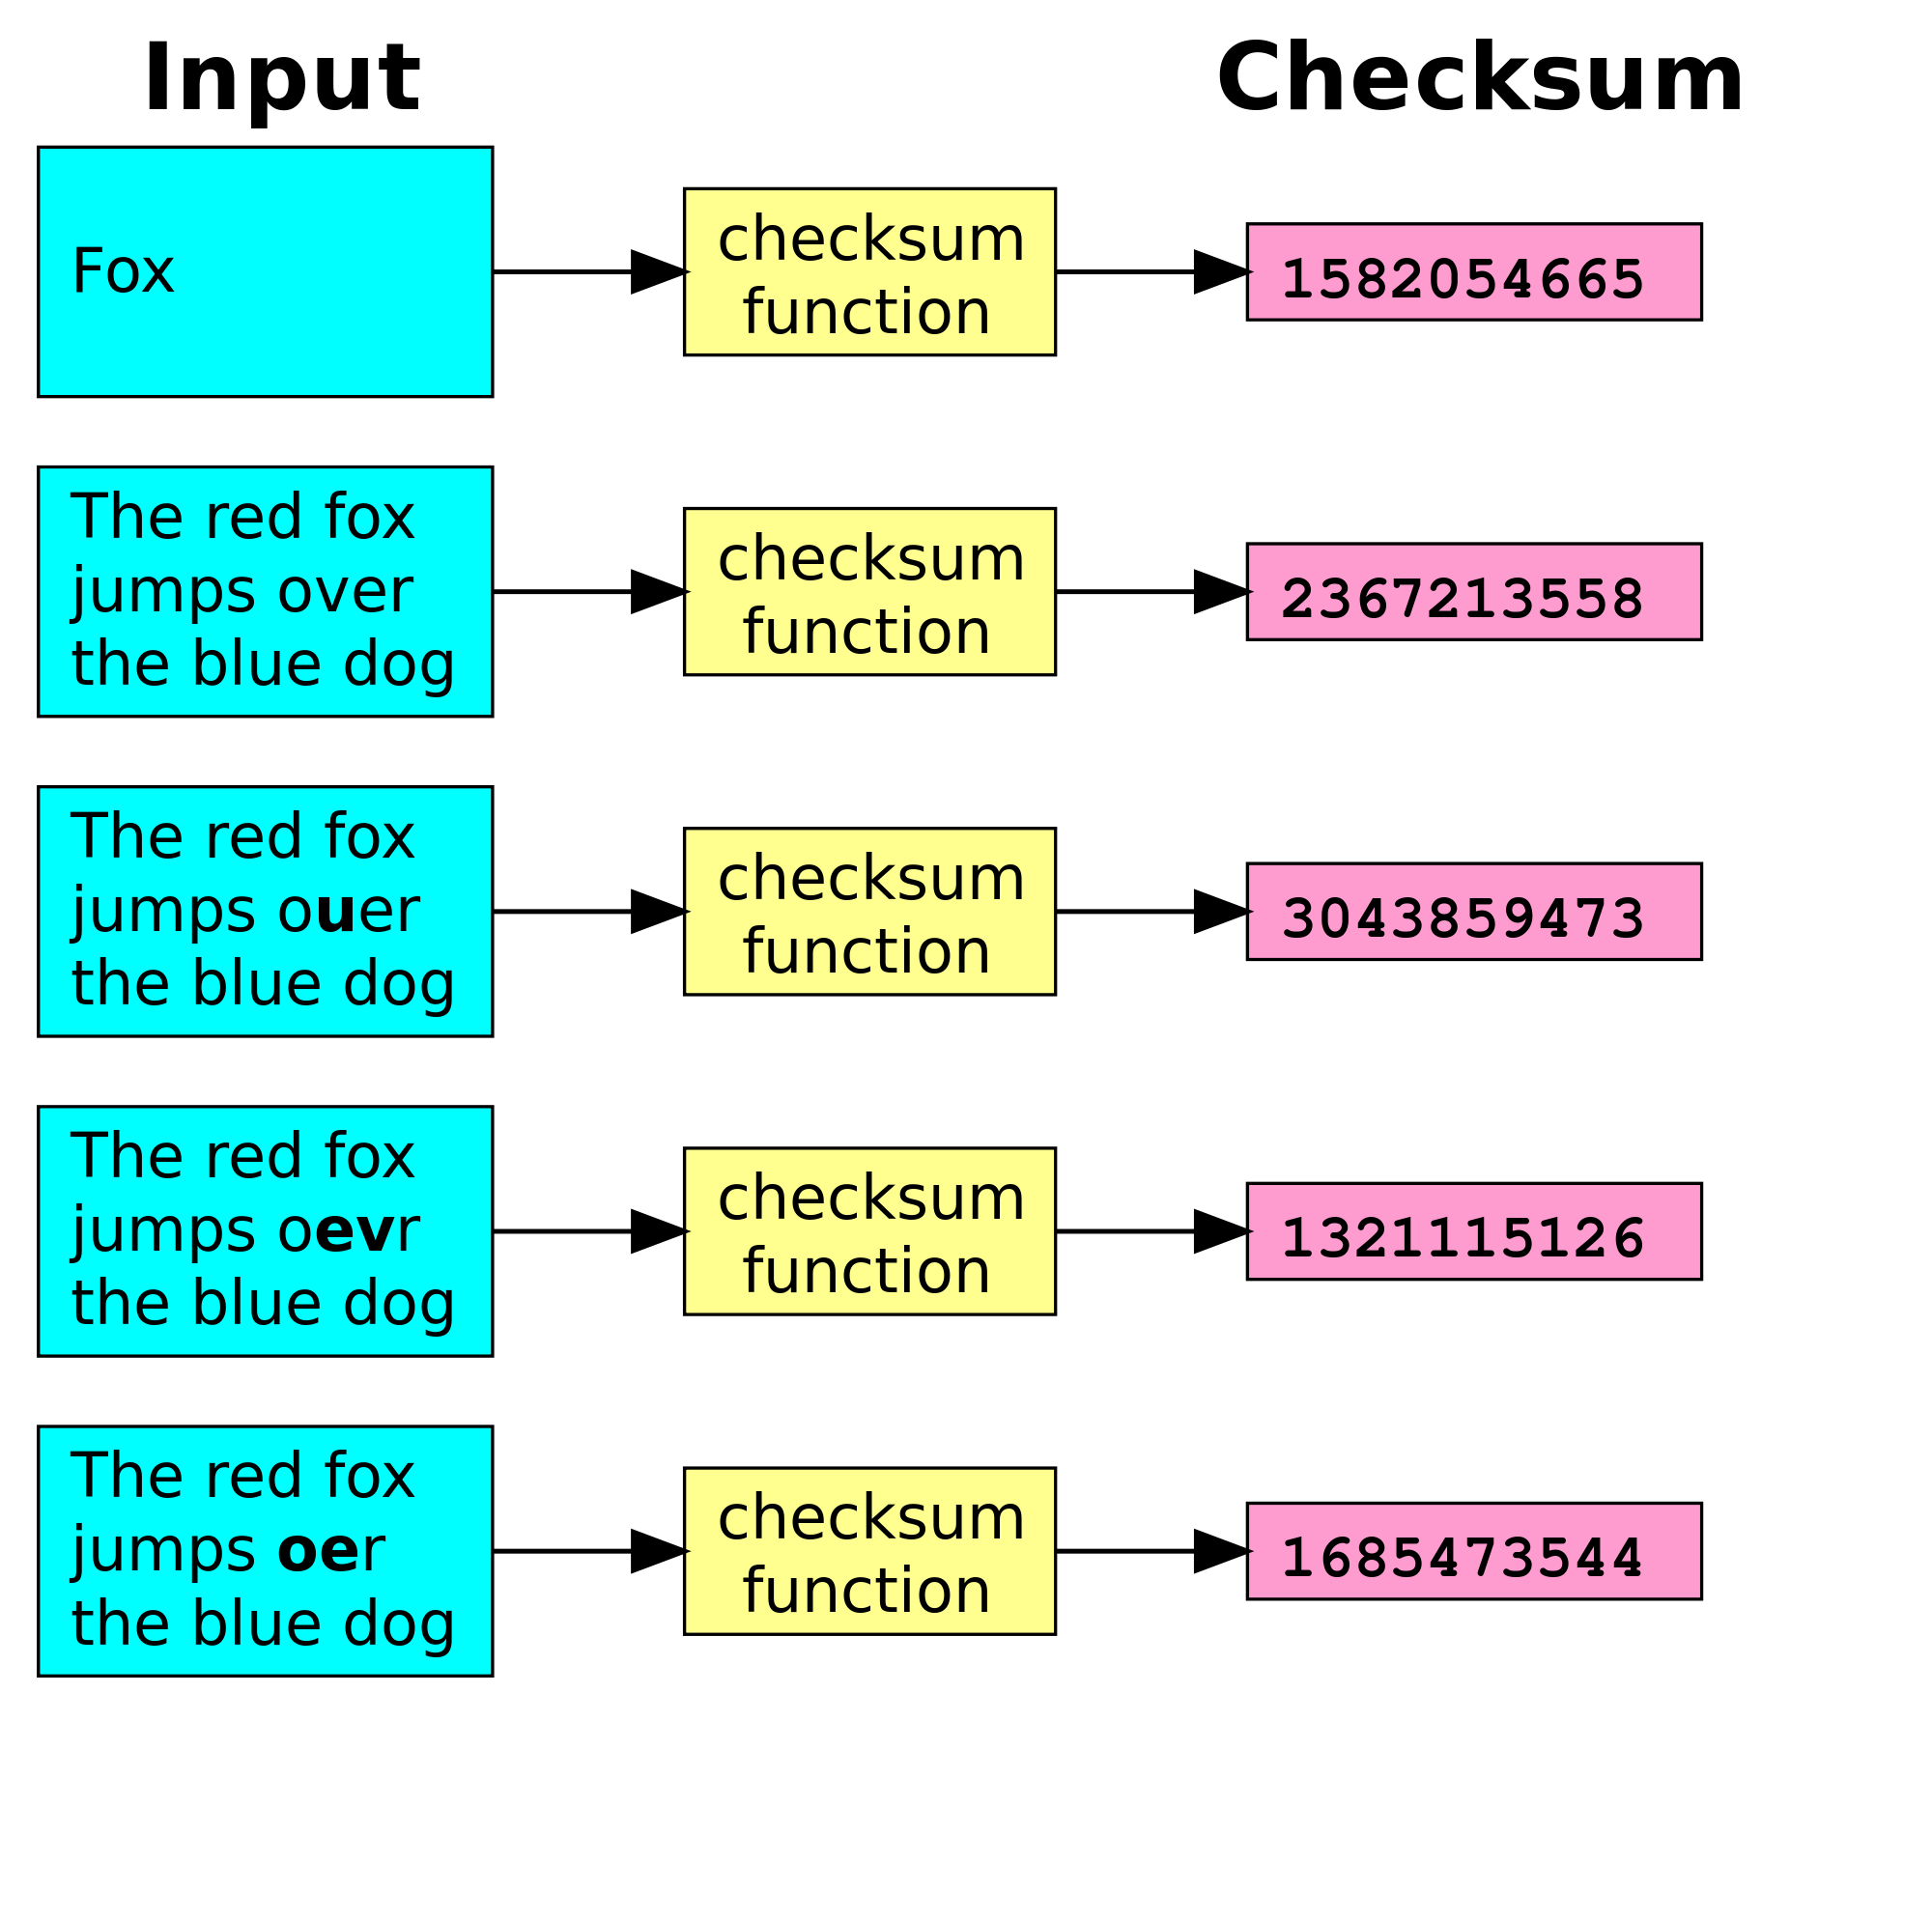
\includegraphics[width=0.35\textwidth]{checksum.png} 
\end{center}
\end{frame}


\section{Implementação de um sistema de montagem de disco exFAT}
\begin{frame}[fragile]{exFAT root}
\begin{lstlisting}
struct exfat
{
	struct exfat_dev* dev;
	struct exfat_super_block* sb;
	le16_t* upcase;
	size_t upcase_chars;
	struct exfat_node* root;
	struct
	{
		cluster_t start_cluster;
		uint32_t size;				/* in bits */
		bitmap_t* chunk;
		uint32_t chunk_size;		/* in bits */
		bool dirty;
	}
	cmap;
	char label[UTF8_BYTES(EXFAT_ENAME_MAX) + 1];
	void* zero_cluster;
	int dmask, fmask;
	uid_t uid;
	gid_t gid;
	int ro;
	bool noatime;
};
\end{lstlisting}
https://code.google.com/p/exfat/
\end{frame}

\begin{frame}[fragile]{Node de exFAT}
\begin{lstlisting}
struct exfat_node {
	struct exfat_node* parent;
	struct exfat_node* child;
	struct exfat_node* next;
	struct exfat_node* prev;

	int references;
	uint32_t fptr_index;
	cluster_t fptr_cluster;
	cluster_t entry_cluster;
	off_t entry_offset;
	cluster_t start_cluster;
	int flags;
	uint64_t size;
	time_t mtime, atime;
	le16_t name[EXFAT_NAME_MAX + 1];
};
\end{lstlisting}
https://code.google.com/p/exfat/
\end{frame}



\begin{frame}{Restrictive licensing and software patents}

A micro$\$$oft não liberou oficialmente as especificações do sistema de arquivos exFAT e deixou este com uma licensa restritiva, a qual é necessaria para fazer e distribuir implementações completas do sistema exFAT. A micro$\$$oft ainda reinvidica algumas patentens de softwares que torna dificil reimplementar todas as funcionalidades requeridas pelo sistema de arquivos exFAT sem violar uma muitas destas pastentes.

Isso torna a implementação, distribuição e uso do exFAT como parte daa comunidade livre de sistemas de codigo livre e softwares comerciais dificil, para vendedores que não conseguem obter a licensa da micro$\$$oft,  especialmente em paises que reconhecem as patentes de Software dos Estados Unidos.
\end{frame}

\begin{frame}{Restrictive licensing and software patents}
Apesar do sistema exFAT ser amplamente suportado atualmente, em dispositivos eletronicos e Mac OS X, inicialmente ses so podiam lidar com formatos FAT12/FAT16/FAT32, o que tornava o exFAT impraticavel como um sistema universal de armazenamento de dados. 

O suporte para o exFAT em sistemas linux ainda é limitado devido a essas barreiras.
\end{frame}





\end{document}

